% Options for packages loaded elsewhere
\PassOptionsToPackage{unicode}{hyperref}
\PassOptionsToPackage{hyphens}{url}
%
\documentclass[
]{article}
\usepackage{amsmath,amssymb}
\usepackage{iftex}
\ifPDFTeX
  \usepackage[T1]{fontenc}
  \usepackage[utf8]{inputenc}
  \usepackage{textcomp} % provide euro and other symbols
\else % if luatex or xetex
  \usepackage{unicode-math} % this also loads fontspec
  \defaultfontfeatures{Scale=MatchLowercase}
  \defaultfontfeatures[\rmfamily]{Ligatures=TeX,Scale=1}
\fi
\usepackage{lmodern}
\ifPDFTeX\else
  % xetex/luatex font selection
\fi
% Use upquote if available, for straight quotes in verbatim environments
\IfFileExists{upquote.sty}{\usepackage{upquote}}{}
\IfFileExists{microtype.sty}{% use microtype if available
  \usepackage[]{microtype}
  \UseMicrotypeSet[protrusion]{basicmath} % disable protrusion for tt fonts
}{}
\makeatletter
\@ifundefined{KOMAClassName}{% if non-KOMA class
  \IfFileExists{parskip.sty}{%
    \usepackage{parskip}
  }{% else
    \setlength{\parindent}{0pt}
    \setlength{\parskip}{6pt plus 2pt minus 1pt}}
}{% if KOMA class
  \KOMAoptions{parskip=half}}
\makeatother
\usepackage{xcolor}
\usepackage[margin=1in]{geometry}
\usepackage{graphicx}
\makeatletter
\def\maxwidth{\ifdim\Gin@nat@width>\linewidth\linewidth\else\Gin@nat@width\fi}
\def\maxheight{\ifdim\Gin@nat@height>\textheight\textheight\else\Gin@nat@height\fi}
\makeatother
% Scale images if necessary, so that they will not overflow the page
% margins by default, and it is still possible to overwrite the defaults
% using explicit options in \includegraphics[width, height, ...]{}
\setkeys{Gin}{width=\maxwidth,height=\maxheight,keepaspectratio}
% Set default figure placement to htbp
\makeatletter
\def\fps@figure{htbp}
\makeatother
\setlength{\emergencystretch}{3em} % prevent overfull lines
\providecommand{\tightlist}{%
  \setlength{\itemsep}{0pt}\setlength{\parskip}{0pt}}
\setcounter{secnumdepth}{-\maxdimen} % remove section numbering
\ifLuaTeX
  \usepackage{selnolig}  % disable illegal ligatures
\fi
\IfFileExists{bookmark.sty}{\usepackage{bookmark}}{\usepackage{hyperref}}
\IfFileExists{xurl.sty}{\usepackage{xurl}}{} % add URL line breaks if available
\urlstyle{same}
\hypersetup{
  pdftitle={Quiz1},
  hidelinks,
  pdfcreator={LaTeX via pandoc}}

\title{Quiz1}
\author{}
\date{\vspace{-2.5em}2024-02-15}

\begin{document}
\maketitle

\textbf{Problem 1}
\includegraphics{Quiz1_files/figure-latex/unnamed-chunk-1-1.pdf}

\begin{verbatim}
## Mean: 169.9048
\end{verbatim}

\begin{verbatim}
## 0.68-Quantile: 175
\end{verbatim}

\begin{verbatim}
## Q1: 165
\end{verbatim}

\begin{verbatim}
## Q2 (Median): 171
\end{verbatim}

\begin{verbatim}
## Q3: 177
\end{verbatim}

\begin{verbatim}
## Outliers: 126
\end{verbatim}

\textbf{Problem 2}
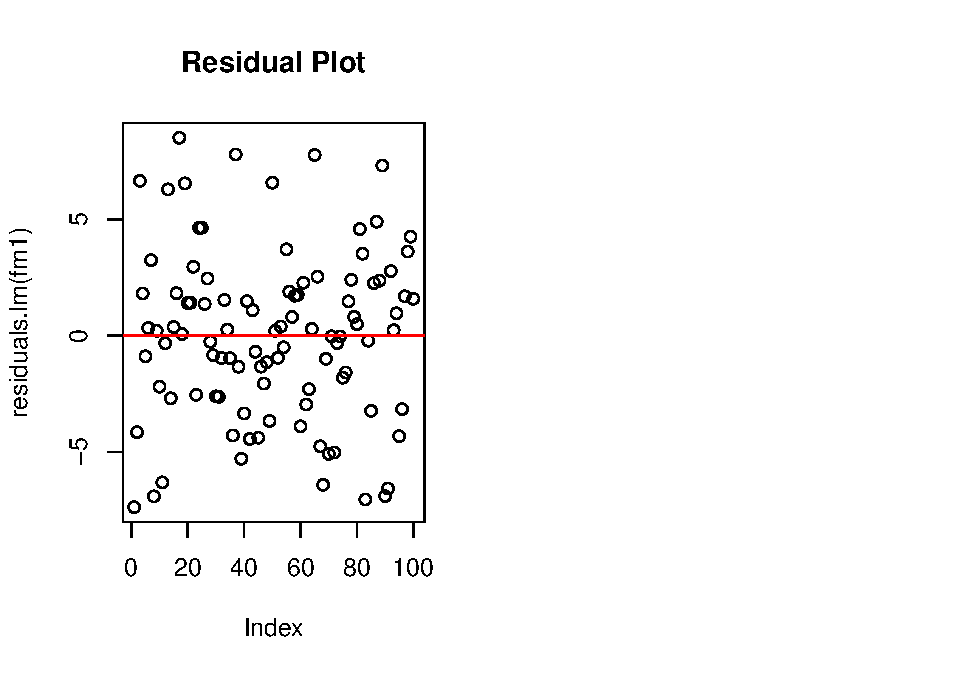
\includegraphics{Quiz1_files/figure-latex/unnamed-chunk-2-1.pdf}

\begin{verbatim}
## IQR: 12
\end{verbatim}

\begin{verbatim}
## Variance: 168.4905
\end{verbatim}

\begin{verbatim}
## Standard Deviation: 12.98039
\end{verbatim}

\begin{verbatim}
## Mean: 169.9048
\end{verbatim}

\begin{verbatim}
## Median: 171
\end{verbatim}

\begin{verbatim}
## The distribution is negatively skewed.
\end{verbatim}

\textbf{Problem 3}\\
\textbf{i}

\begin{verbatim}
## Observed value t1: 130.5769
\end{verbatim}

\begin{verbatim}
## P(|T1| <= |t1|): 1
\end{verbatim}

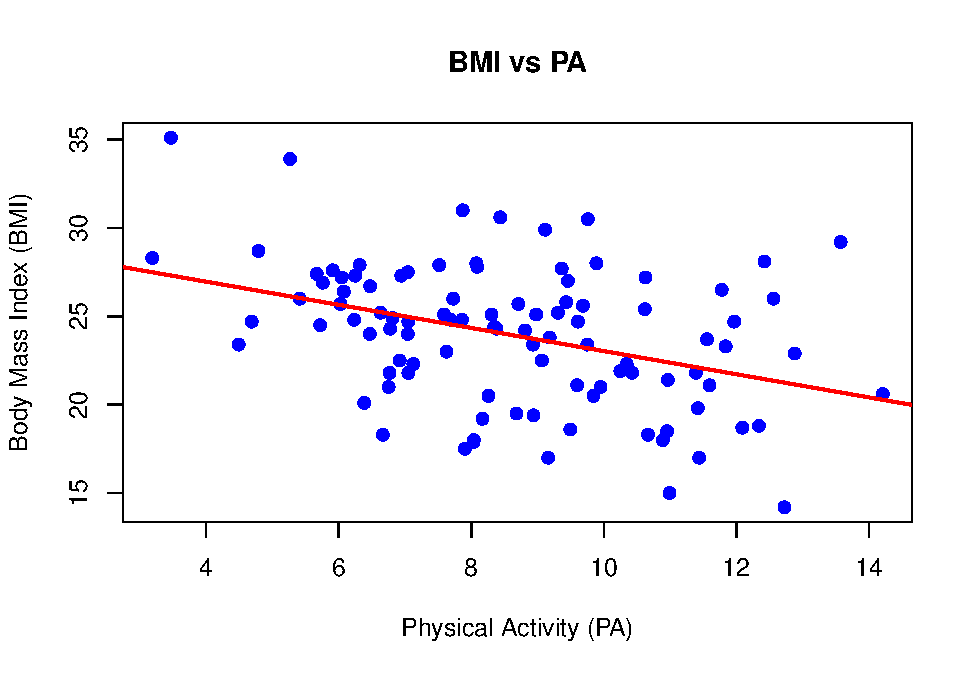
\includegraphics{Quiz1_files/figure-latex/unnamed-chunk-3-1.pdf}

\textbf{ii}

\begin{verbatim}
## Observed value t2: 129.6081
\end{verbatim}

\begin{verbatim}
## P(|T2| <= |t2|): 1
\end{verbatim}

\includegraphics{Quiz1_files/figure-latex/unnamed-chunk-4-1.pdf}

\textbf{iii}

No they are not different because both are calculated based on
chi-square distributions.

\textbf{iv}

t-distribution t3 = -0.984309 P(T3\textgreater t3) = 0.8316388

\textbf{v}

student t-distribution t4 = -0.38666112 P(T4\textgreater t4) = 0.648454

\textbf{Problem 4}

\begin{enumerate}
\def\labelenumi{\roman{enumi})}
\tightlist
\item
  Linear Combination of Normal Random Variables
\item
  Sum of Scaled Chi-Squared Random Variables
\item
  Ratio of Normal to Square Root of a Weighted Sum of Chi-Squared
  Variables
\item
  Ratio of Two Chi-Squared Variables
\end{enumerate}

\textbf{Problem 5}

\begin{enumerate}
\def\labelenumi{\roman{enumi})}
\item
\item
  The first one is a normal distribution N(0,1) The second one is a
  chi-squared distribution.
\item
\end{enumerate}

The mathematical expectation of the first one is σ2 and for the second
one the (n-1)/n σ2

\begin{enumerate}
\def\labelenumi{\roman{enumi})}
\setcounter{enumi}{2}
\tightlist
\item
  They are not independent and uncorellated because the covariance
  between mu squared and σ2 is zero.
\end{enumerate}

\end{document}
